\documentclass[12pt]{article}

\usepackage{amsmath}
\usepackage{graphicx}

\renewcommand{\contentsname}{Table of Contents}

\begin{document}


\title{Experiment 2.2\\Wheatstone Bridge}
\author{Justin B, Aditya D}
\date{October 24, 2019}
\maketitle

\pagenumbering{roman}
\newpage
\tableofcontents
\newpage 
\pagenumbering{arabic}

\section{Objectives}
In this experiment, we explore the basic principles of the Wheatstone Bridge.
A combination of available resistors, potentiometers, and a force gauge were used to construct a balanced Wheatstone Bridge.
Next, we analyze the relationship between the force applied and the observed output voltage to prove the validity of equation 13 \cite{labManual}.
We comment on the experimental results, possible sources of error, and how to mitigate said errors in future experiments.

\section{Experimental Results}
\paragraph*{}
Using 5 different masses, the following output voltages were obtained (Table \ref{table:1}).

\begin{table}[h]
\centering
\begin{tabular}{c | c }
    Force (\(N\)) & Voltage (\(V\)) \\
    \hline
    1.226 & 0.167 \\
    1.275 & 0.176 \\
    1.271 & 0.182 \\
    1.238 & 0.180 \\
    1.245 & 0.176 \\
\end{tabular}
\caption{Force versus Voltage across bridge}
\label{table:1}
\end{table}

Graphing the data points from (Table \ref{table:1}), we obtain the gain of the apparatus as \(\frac{0.1355V}{1N}\) (Figure \ref{Figure 1}).

\begin{figure}[ht]
    \centering
    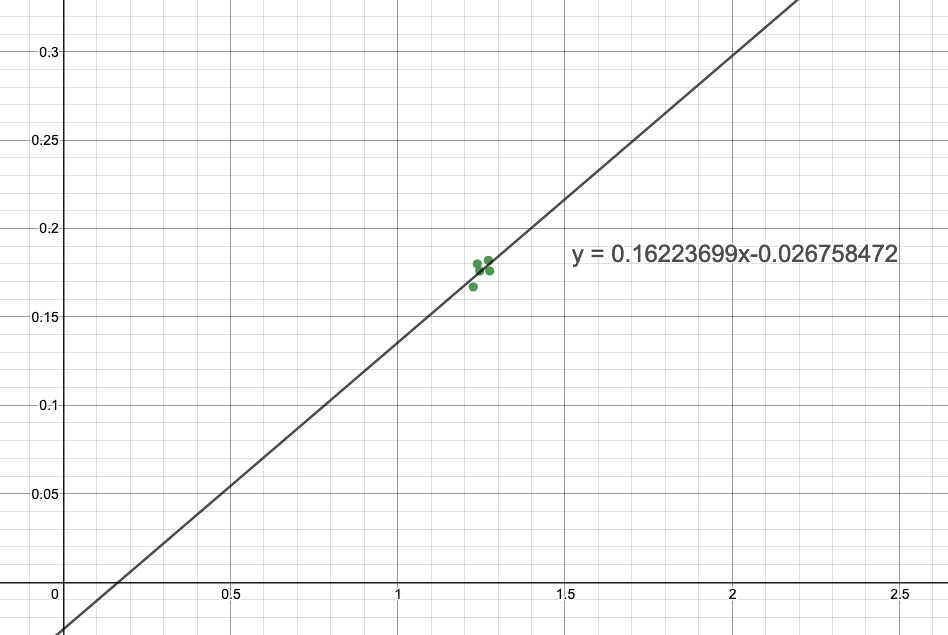
\includegraphics[height=9cm]{linear_relation.png}
    \caption{Output voltage ($V$) versus force ($N$) with $r^2 = 0.358$.}
    \label{Figure 1}
\end{figure}

\section{Discussion}
As labeled in Figure 12 \cite{labManual}, the following values were chosen/measured:
\begin{align*}
    E   &= 12.0V \\
    R_1 &= 100\Omega \\
    R_2 &= 910\Omega \\
    R_3 &= 0\!-\!200\Omega \\
    R_x &= 960.7\Omega 
\end{align*}

For a balanced bridge, \(R_1R_x = R_2R_3\), and the chosen configuration of resistors satisfies this condition.
\begin{align*}
    \left(100\Omega\right)\left(960.7\Omega\right) = \left(910\Omega\right)\left(106\Omega\right) 
\end{align*}

\paragraph*{}
The \(200\Omega\) potentiometer was chosen because the bridge is balanced when it has a resistance of \(106\Omega\), allowing for maximal variation.

\paragraph*{}
Using the graph in (Figure \ref{Figure 1}), the gain is calculated as \(\frac{0.1355V}{1N}\).

\paragraph*{}
The relation between the output voltage and the applied force was roughly linear, as predicted by equation 13 \cite{labManual}.
A large factor contributing to variance in the data was the force sensor's resistance drifting over time which made it difficult to obtain precise data points without waiting for the drift to slow down.
The variance in the data could be reduced by using a more sensitive potentiometer to allow for more accurate calibration and by using a force sensor with less drift.

\section{Conclusion}
The constructed Wheatstone Bridge demonstrated the predicted linear relationship between the output voltage and the sensor resistance.
Using a sufficiently sensitive potentiometer allows the bridge to be balanced under no load, and thus accurately relate the output voltage to the applied force.


\newpage
\addcontentsline{toc}{section}{References}
\begin{thebibliography}{1}
    \bibitem{labManual}
    N. Dimopoulos, F. Gebali, \textit{Laboratory Manual: ECE 250, \\ Linear Circuits I (Edition 4)}, University of Victoria, Victoria, B.C, 2018, pp.19-23.
\end{thebibliography}

\end{document}